% !TeX root = ./FAN-T2-relatorio.tex
\documentclass[brazil, a4paper, 12pt]{article}

% █▀█ █▀█ █▀▀ ▄▀█ █▀▄▀█ █▄▄ █   █▀▀
% █▀▀ █▀▄ ██▄ █▀█ █ ▀ █ █▄█ █▄▄ ██▄

%::::::::::::::::::::::::::::::::::::::::::::::::::::::::::::::::::::::::::::::::
%                                   CORE SETUP                                   
%                             Document-Wide Settings                             
%................................................................................
\usepackage[
	a4paper,
	margin=2cm,
]{geometry}	% Set page margins
\usepackage[brazil]{babel}		% Language-specific settings
\usepackage{csquotes}			% Context-sensitive quoting
					% 'csquotes' works in tandem with babel
					% 'csquotes' IS A 'biblatex' DEPENDENCY

%::::::::::::::::::::::::::::::::::::::::::::::::::::::::::::::::::::::::::::::::
%                               MATH & FONT ENGINE                               
%................................................................................
% AMS (American Mathematical Society)
\usepackage{amsmath}		% AMS's package for mathematical typesetting
\usepackage{mathtools}		% Extends amsmath's functionalities (i.e.: a superset)
\usepackage{amsthm}		% AMS's package for creating theorem-like environments

\usepackage{fontspec}		% Interface for using system fonts (OTF/TTF) with Lua/XeLaTeX
\usepackage[
	math-style = ISO,
	bold-style = ISO
]{unicode-math}	% Must be loaded after 'mathtools'

% Font selection
\setmainfont{Libertinus Serif}
\setsansfont{Libertinus Sans}[
	BoldItalicFont = {Libertinus Sans Italic} % Fallback for missing BI
]
\setmonofont{Libertinus Mono}[
	BoldFont		= {Libertinus Mono},	% Fallback for missing B
	ItalicFont		= {Libertinus Mono},	% Fallback for missing I
	BoldItalicFont	= {Libertinus Mono}	% Fallback for missing BI
]
\setmathfont{Libertinus Math}
\setmathfont[range=\mathcal, StylisticSet=1]{XITS Math}	% Libertinus uses a single font for both script and calligraphic text
\setoperatorfont{\mathsf}	% Sans (without) serif font to distinguish mathematical operators from prose
%::::::::::::::::::::::::::::::::::::::::::::::::::::::::::::::::::::::::::::::::
%                                    STYLING                                     
%                        Alter Visual Appearance of Text                         
%................................................................................
\usepackage{microtype}		% Enhance micro-typography (e.g.: protrusion, expansion)
\usepackage{fancyhdr}		% Custom headers and footers
\pagestyle{plain}		% header: empty; footer: centered page number
\usepackage[dvipsnames]{xcolor}	% Access to 68 named colors
\usepackage{moresize}		% Additional font sizes
\usepackage{enumerate}		% Customize item style in 'enumerate'
\usepackage{multicol}		% Environment with multiple columns of text
\usepackage[normalem]{ulem}	% More underline styles (and aligns bottoms of multiple underlines)
				% 'normalem' prevents underlines from altering \emph
\usepackage{appendix}		% Provides an 'appendices' environment for easy formatting
\usepackage{romannum}		% Adds romam numbers


%::::::::::::::::::::::::::::::::::::::::::::::::::::::::::::::::::::::::::::::::
%                                     FLOATS                                     
%               Manage Floating Content (e.g.: figures and tables)               
%................................................................................
\usepackage{subcaption}	% Format multiple images(tables) in one figure(table) environment
			% NOTE: This package *automatically* loads the 'caption' package,
\captionsetup{
	labelfont = {small,bf},
	textfont  = {small,it}
}
%\subcaptionsetup{...}	% Uncomment to customize sub-captions separately

\usepackage{booktabs}	% Format tables following scientific convention
\usepackage{float}	% Provides [H] 'Here' float placement specifier (use with caution)


%:::::::::::::::::::::::::::::::::::::::::::::::::::::::::::::::::::::::::::::::::
%                                    GRAPHICS                                    
%                             Generate/Import Images                              
%.................................................................................
% NATIVE PROGRAMMATIC DIAGRAMS & PLOTS
\usepackage{tikz}		% Create vector graphics programmatically
\usetikzlibrary{arrows.meta}	% Additional arrow styles
\usepackage{pgfplots}		% Tool for creating function plots and charts
\pgfplotsset{compat=1.18}	% Enforce version 1.18 for consistency

% EXTERNAL IMAGE MANAGEMENT
\usepackage{graphicx}		% LaTeX standard for including external image files


% █▀▄▀█ ▄▀█ ▀█▀ █ █
% █ ▀ █ █▀█  █  █▀█
%:::::::::::::::::::::::::::::::::::::::::::::::::::::::::::::::::::::::::::::::::
%                                 MATH PACKAGES                                  
%.................................................................................
% ALGORITHMS
\usepackage[
	portuguese,
	ruled,
	vlined,
	linesnumbered
]{algorithm2e}	% Typeset formal algorithms
\SetKwInput{KwRequer}{Requer}
\SetKwInput{KwPrecondicao}{Pré-condição}
\SetKwInput{KwInicializa}{Inicializa}
\SetKwFor{Para}{para}{faça}{fim para}
\SetKwIF{Se}{SenaoSe}{Senao}{se}{então}{senão se}{senão}{fim se}
\DontPrintSemicolon

% NICHE MATH PACKAGES
\usepackage{xfrac}	% Slanted fractions (\sfrac)
\usepackage{cancel}	% Strike-through for symbols (\cancel and \cancelto)
\usepackage{bbm}	% Shorthand solution for blackboard boldfaced 1 (use \mathbbm{1})

%::::::::::::::::::::::::::::::::::::::::::::::::::::::::::::::::::::::::::::::::::
%                           CUSTOM THEOREM ENVIRONMENTS                            
%                                   (Color Coded)                                  
%..................................................................................
% 1. DEFINE COLOR CODE FOR EACH THEOREM-LIKE ENVIRONMENT (makes change of color choice effortless)
\colorlet{lmm}{DarkOrchid}	% For lemma env.
\colorlet{thm}{Tan}		% For theorem env.
\colorlet{prop}{Maroon}		% For proposition env.
\colorlet{crl}{RawSienna}	% For corollary env.
\colorlet{def}{OliveGreen}	% For definition env.
\colorlet{eg}{RoyalPurple}	% For example env.
\colorlet{ex}{RoyalPurple}	% For exercise env.
\colorlet{obs}{MidnightBlue}	% For remark env.
\colorlet{note}{PineGreen}	% For notation remark env.

%. . . . . . . . . . . . . . . . . . . . . . . . . . . . . . . . . . . . . . . . . 
% 2. DEFINE CUSTOM THEOREM STYLES
% 2.1. STYLE I - TAUTOLOGIES - FIRST NUMBER, THEN NAME
\newtheoremstyle{number-name}
{4mm}						% Space above env.
{4mm}						% Space below env.
{\itshape}					% Body font
{}						% Indent amount
{\bfseries}					% Head font
{:}						% Punctuation after head
{.3em}						% Space after head
{\thmnumber{#2}\,\thmname{#1}\thmnote{ (#3)}}	% Head spec

% 2.2. STYLE II - EXAMPLES & EXERCISES - FIRST NAME, THEN ITALIC NUMBER 
\newtheoremstyle{name-it_number}
{4mm}						% Space above env.
{4mm}						% Space below env.
{\itshape}					% Body font
{}						% Indent amount
{\bfseries}					% Head font
{}						% Punctuation after head
{.3em}						% Space after head
{\thmname{#1}\,{\itshape\thmnumber{#2}}}	% Head spec

% 2.3. STYLE III - REMARKS, SOLUTIONS & PROOFS - NO NUMBERING (should refer to a numbered env.)
\newtheoremstyle{no_number}
{4mm}						% Space above env.
{4mm}						% Space below env.
{}						% Body font
{}						% Indent amount
{\bfseries\itshape}				% Head font
{.}						% Punctuation after head
{.3em}						% Space after head
{}						% Head spec

% 2.4. STYLE IV - NOTATION REMARKS - NO NUMBERING (should refer to a numbered env.) AND ITALIC BODY 
\newtheoremstyle{no_number-it_body}
{4mm}						% Space above
{4mm}						% Space below
{\itshape}					% Body font
{}						% Indent amount
{\bfseries}					% Head font
{:}						% Punctuation after head
{.3em}						% Space after head
{}						% Head spec

%. . . . . . . . . . . . . . . . . . . . . . . . . . . . . . . . . . . . . . . . .
% 3. APPLY THEOREM STYLES AND DEFINE RESPECTIVE ENVIRONMENTS
% 3.1. STYLE I - TAUTOLOGIES - FIRST NUMBER, THEN NAME
\theoremstyle{number-name}
  \newtheorem{lemma}{\color{lmm}Lema}[section]
  \newtheorem{theorem}{\color{thm}Teorema}[section]
  \newtheorem{proposition}{\color{prop}Proposição}[section]
  \newtheorem{corollary}{\color{crl}Corolário}[section]
  \newtheorem{definition}{\color{def}Definição}[section]

% Manually force counters to share the 'lemma' counter (i.e.: shared counter for style I)
\makeatletter
\let\c@theorem\c@lemma
\let\c@proposition\c@lemma
\let\c@corollary\c@lemma
\let\c@definition\c@lemma
\makeatother

% 3.2. STYLE II - EXAMPLES & EXERCISES - FIRST NAME, THEN ITALIC NUMBER 
\theoremstyle{name-it_number}
  \newtheorem{exercise}{\textcolor{ex}{Exercício}}[section]
  \newtheorem{example}{\textcolor{eg}{Exemplo}}[section]

% Manually force 'example' to use the 'exercise' counter (i.e. shared counter for style II)
\makeatletter
\let\c@example\c@exercise
\makeatother

% 3.3. STYLE III - REMARKS, SOLUTIONS & PROOFS - NO NUMBERING
\theoremstyle{no_number}
  % Remark
  \newtheorem*{observation*}{\color{obs}Observação}
  % Solution
  \newtheorem*{solution}{\color{ex}Solução}
  % Proofs
  \newtheorem*{proofT}{\color{thm}Demonstração}
  \newtheorem*{proofL}{\color{lmm}Demonstração}
  \newtheorem*{proofC}{\color{crl}Demonstração}
  \newtheorem*{proofP}{\color{prop}Demonstração}
  \newtheorem*{proofE}{\color{eg}Demonstração}
  \newtheorem*{proofO}{\color{obs}Demonstração}

% 3.4. STYLE IV - NOTATION REMARKS - NO NUMBERING AND ITALIC BODY 
\theoremstyle{no_number-it_body}
  \newtheorem*{notation*}{\color{note}Notação}

%. . . . . . . . . . . . . . . . . . . . . . . . . . . . . . . . . . . . . . . . .
% EXTRA: CUSTOM QED SYMBOL (a small black square)
\renewcommand\qedsymbol{■}


%:::::::::::::::::::::::::::::::::::::::::::::::::::::::::::::::::::::::::::::::::
%                              CUSTOM MATH COMMANDS                               
%.................................................................................
\newcommand{\Bvec}[1]{\symbf{#1}}	% Bold symbol vector notation

% CONSTANTS
\newcommand{\e}{\mathscr{e}}		% Special notation for Euler's number
\newcommand{\im}{\mathscr{i}\,}		% Special notation for the imaginary unit

% RELATIONS
\newcommand{\longto}{\longrightarrow}	% Alias to note function domain/codomain (f: A --> B)

% Bellow, a colon-equals (and an analogous equals-colon) sign built 'from scratch', to be more compact and elegant
\newcommand*{\Defeq}{%
	\mathrel{%						% Wrapper so TeX treats/interprets the symbol as a relation
		\vcenter{%					% Vertically center the 'colon' part
			\baselineskip0.5ex%			% Manually set the vertical spacing between the dots
			\lineskiplimit0pt%			% Disable TeX's 'anti-collision' rule for full control
			\hbox{\scriptsize.}%			% The top dot
			\hbox{\scriptsize.}%			% The bottom dot
		}%
		{=}%						% The equals sign
	}%
}					% Compact colon-equals
\newcommand*{\Eqdef}{%
	\mathrel{%						% Wrapper so TeX treats/interprets the symbol as a relation
		{=}%						% The equals sign
		\vcenter{%					% Vertically center the 'colon' part
			\baselineskip0.5ex%			% Manually set the vertical spacing between the dots
			\lineskiplimit0pt%			% Disable TeX's 'anti-collision' rule for full control
			\hbox{\scriptsize.}%			% The top dot
			\hbox{\scriptsize.}%			% The bottom dot
		}%
	}%
}					% Compact equals-colon
\newcommand{\subnormal}{\triangleleft}	% Normal subgroup (left)
\newcommand{\supnormal}{\triangleright}	% Normal subgroup (right)

% UNARY OPERATIONS
\newcommand{\T}{{\mathsfup{T}}}				% Transpose symbol
\newcommand{\Tp}[1]{{#1}^{\mathsfup{T}}}	% Transpose operation

% LOGIC
\newcommand{\limplies}{\rightarrow}	% Conditional connector
\newcommand{\liff}{\leftrightarrow}	% Biconditional connector
\newcommand{\nand}{\uparrow}		% NAND connector
\newcommand{\nor}{\downarrow}		% NOR connector
\newcommand{\xor}{\veebar}		% XOR connector


% LOADED LAST TO AVOID DEPENDENCY ERRORS
%:::::::::::::::::::::::::::::::::::::::::::::::::::::::::::::::::::::::::::::::::
%                                  BIBLIOGRAPHY                                   
%                                Manage References                                
%.................................................................................
\usepackage[
	backend=biber,	% Use Biber backend (more powerful than BibTex)
	style=ieee,
	backref=true
]{biblatex}


%:::::::::::::::::::::::::::::::::::::::::::::::::::::::::::::::::::::::::::::::::
%                                  FINALIZATION                                   
%                 Packages That Patch Others. MUST BE LOADED LAST                 
%.................................................................................
\usepackage{hyperref}		% Add hyperlinks to references, ToC and URLs
\hypersetup{
	plainpages=false,	% Try to prevent duplicate page anchors
	colorlinks=true,	% true: colored links; false: boxed links
	linkcolor=NavyBlue,	% Internal links
	citecolor=NavyBlue,
	urlcolor=NavyBlue,
	breaklinks=true,
	pdfborder={0 0 0}
}

\usepackage[
	brazilian,
	nameinlink
]{cleveref}			% Objectively better than \autoref
% DEFINE 'cleveref' NAMES FOR CUSTOM THEOREM-LIKE ENVIRONMENTS
	% STYLE I ENVIRONMENTS
\crefname{lemma}{lema}{lemas}
\Crefname{lemma}{Lema}{Lemas}
\crefname{theorem}{teorema}{teoremas}
\Crefname{theorem}{Teorema}{Teoremas}
\crefname{proposition}{proposição}{proposições}
\Crefname{proposition}{Proposição}{Proposições}
\crefname{corollary}{corolário}{corolários}
\Crefname{corollary}{Corolário}{Corolários}
\crefname{definition}{definição}{definições}
\Crefname{definition}{Definição}{Definições}
	% STYLE II ENVIRONMENTS
\crefname{exercise}{exercício}{exercícios}
\Crefname{exercise}{Exercício}{Exercícios}
\crefname{example}{exemplo}{exemplos}
\Crefname{example}{Exemplo}{Exemplos}

\newcommand{\customref}[2]{%	% Simple alias for custom link text
	\hyperref[#2]{#1}%
}


\addbibresource{bib-relatorio.bib}
\graphicspath{ {../plots/} }

\title{Estatística descritiva sobre um conjunto de dados}
\author{Kainã Alves Tureso - 15466391\\
        Pedro Luís Anghievisck - 15656521}
\date{\today}

\begin{document}
    \maketitle
    \tableofcontents
    \break

    \section{Dados}
    Os dados foram retirados de \cite{cars_data}, mas estavam originalmente no repositório \textit{StatLib}, mantido pela Universidade Carnegie Mellon. Esse conjunto foi utilizado na exposição de 1983 da Associação Americana de Estatística. Nele, se encontram informações (como número de cilindros, potência, aceleração, peso, etc.) sobre modelos de carros das décadas de 70 e 80 que foram produzidos no Japão, Europa e Estados Unidos.

    Para esse estudo foram selecionadas as seguintes variáveis:
    \begin{itemize}
        \item \textbf{Qualitativa:} local de produção;
        \item \textbf{Quantitativa contínua:} aceleração;
        \item \textbf{Quantitativa discreta:} número de cilindros do motor.
    \end{itemize}

    A amostra continha $n=398$ observações, todas sem nenhuma variável sem valor.

    \section{Variável qualitativa}
    Como citado anteriormente, a variável "local de produção" possui três valores únicos diferente, sendo eles "usa", "japan" e "europe". Ao organizar os dados, a seguinte tabela foi montada:
    \begin{table}[H]
        \centering
        \begin{tabular}{c|cc|cc}
            \toprule
            Origem & Frequência & Frequência acumulada & Frequência relativa & Frequência relativa acumulada \\
            \midrule
            usa & 249 & 249 & 0.625628 & 0.625628 \\
            japan & 79 & 328 & 0.198492 & 0.824121 \\
            europe & 70 & 398 & 0.175879 & 1.000000 \\
            \bottomrule
        \end{tabular}

        \caption{Local de produção dos carros}
        \label{table:local_producao}
    \end{table}

    Com isso, podemos construir gráficos da \autoref{fig:graficos_quali} que representem esses dados. O gráfico de setores representa a frequência relativa e o gráfico de barras nos dá uma visualização da frequência absoluta dos dados.
    \begin{figure}[H]
        \centering
        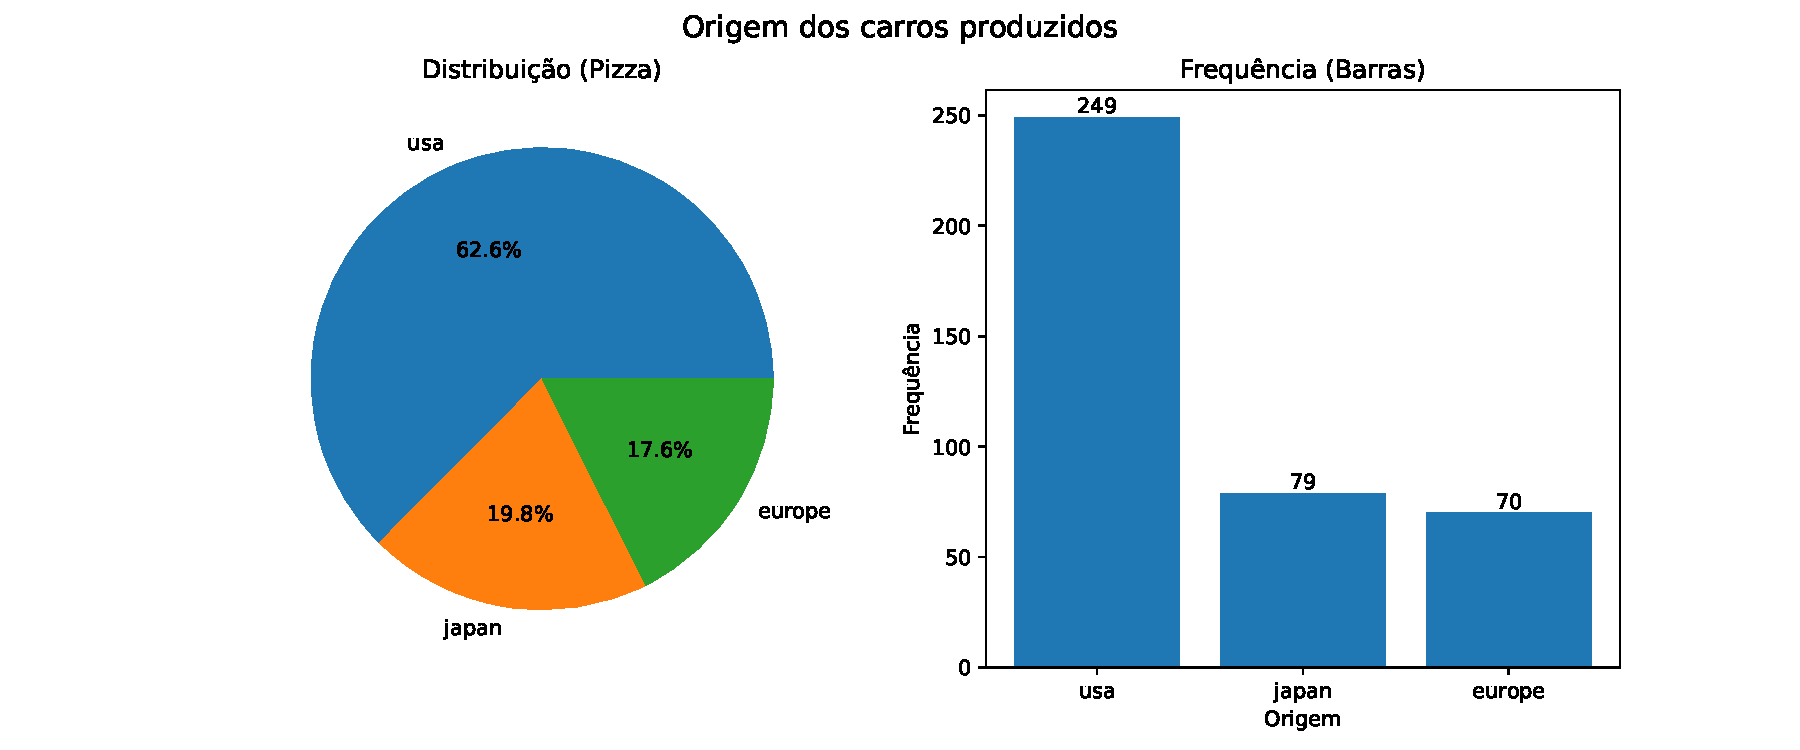
\includegraphics[width=1\textwidth]{plots_quali}
        \caption{Visualização das frequências das origens}
        \label{fig:graficos_quali}
    \end{figure}

    Fica clara a discrepância entre a produção de carros nos EUA e nos outros dois locais (pelo menos para os modelos estudados), com o país americano tendo $62.6\%$ da produção. Em relação às outras origens dos carros do estudo, elas possuem frequências similares, algo peculiar, visto que a Europa é um continente e o Japão um país.

    \section{Variável contínua}
    Para a variável contínua, foi escolhida a aceleração dos carros, medida em milhas por segundo ao quadrado ($mph^2$). Essa medida é obtida fazendo o carro sair do repouso e chegar até $60mph$ e cronometrando o tempo gasto.
    
    Ao observar o rol dessa variável, pode-se encontrar valores entre aproximadamente $5mph^2$ e $25mph^2$. Além disso, obtemos as seguintes estimativas para as medidas de tendência central, sumarizadas na \autoref{table:tendencia_cental_continua}:
    \begin{table}[htbp]
        \centering
        \begin{tabular}{cc}
            \toprule
            Medida de tendência central & Estimativa ($mph^2$)\\
            \midrule
            Média ($\hat{\mu}$)         & $15.568$ \\
            Mediana ($\hat{Me}$)        & $15.500$ \\
            Moda ($\hat{Mo}$)           & $15.000$ \\
            \bottomrule
        \end{tabular}
        \caption{Medidas de tendência central da variável contínua}
        \label{table:tendencia_cental_continua}
    \end{table}

    Como temos que $\hat{\mu} > \hat{Me} > \hat{Mo}$, verificamos uma assimetria à direita, ou seja, a cauda do lado direito é mais alongada. Note que essa assimetria é bem leve, dado que a diferença entre média e mediana é da casa de $1\cdot 10^{-1}$ e a moda também não está muito longe.

    Em relação aos quartis, obtemos os seguinte valores: $Q_1 = 13.825$, $Q_2 = 15.500$, $Q_3 = 17.175$. Logo, metade das acelerações se encontram no intervalo $[13.825, 17.175]$. Os carros fora desse intervalo ou possuem uma aceleração relativamente alta, ou baixa.

    Com relação às medidas de dispersão, temos a \autoref{table:dispersao_continua}.
    \begin{table}[htbp]
        \centering
        \begin{tabular}{cc}
            \toprule
            Medida de dispersão                   & Estimativa ($mph^2$)\\
            \midrule
            Amplitude ($\hat{A}$)                   & $16.800$ \\
            Amplitude interquartílica ($\hat{d_Q}$) & $3.350$ \\
            Desvio-padrão ($\hat{s}$)               & $2.758$ \\
            Coeficiente de variação ($\hat{CV}$)    & $0.177$ \\
            \bottomrule
        \end{tabular}
        \caption{Medidas de dispersão da variável contínua}
        \label{table:dispersao_continua}
    \end{table}
    \newpage
    Sumarizamos os dados na \autoref{table:aceleracao}. Foi necessário separar os dados em classes, dada a quantidade elevada de valores únicos.

    \begin{table}[htbp]
        \centering
        \begin{tabular}{C{2.5cm}|C{2.5cm}C{2.5cm}|C{2.5cm}C{2.5cm}|C{2.5cm}}
            \toprule
            Aceleração & Frequência & Frequência acumulada & Frequência relativa & Frequência relativa acumulada & Ponto Médio do Intervalo \\
            \midrule
            (7.983, 9.68] & 6 & 6 & 0.015075 & 0.015075 & 8.8315 \\
            (9.68, 11.36] & 15 & 21 & 0.037688 & 0.052764 & 10.5200 \\
            (11.36, 13.04] & 50 & 71 & 0.125628 & 0.178392 & 12.2000 \\
            (13.04, 14.72] & 86 & 157 & 0.216080 & 0.394472 & 13.8800 \\
            (14.72, 16.4] & 101 & 258 & 0.253769 & 0.648241 & 15.5600 \\
            (16.4, 18.08] & 71 & 329 & 0.178392 & 0.826633 & 17.2400 \\
            (18.08, 19.76] & 45 & 374 & 0.113065 & 0.939698 & 18.9200 \\
            (19.76, 21.44] & 13 & 387 & 0.032663 & 0.972362 & 20.6000 \\
            (21.44, 23.12] & 7 & 394 & 0.017588 & 0.989950 & 22.2800 \\
            (23.12, 24.8] & 4 & 398 & 0.010050 & 1.000000 & 23.9600 \\
            \bottomrule
        \end{tabular}
        \caption{Aceleração dos carros por intervalos}
        \label{table:aceleracao}
    \end{table}

    Com base na \autoref{table:aceleracao}, podemos encontrar novos valores (menos precisos) para as estimativas, vistos na \autoref{table:medidas_tabela_continua}. Apesar de termos menos precisão com os valores da tabela, as diferenças entre os cálculos são da ordem de $1\cdot 10^{-1}$. Considerando que os dados têm uma amplitude de $16.8$, esse erro é bem pequeno.

    \begin{table}[htbp]
        \centering
        \begin{tabular}{ccc}
            \toprule
            Medidas & Estimativa ($mph^2$) & Módulo da diferença\\
            \midrule
            Média & $15.530$ & $0.038$ \\
            Mediana & $15.419$ & $0.081$ \\
            Moda & $15.560$ & $0.060$ \\
            $Q_1$ & $13.597$ & $0.228$ \\
            $Q_2$ & $15.419$ & $0.081$ \\
            $Q_3$ & $17.358$ & $0.183$ \\
            Desvio-padrão & $2.793$ & $0.035$ \\
            \bottomrule
        \end{tabular}
        \caption{Medidas encontradas com os valores da tabela}
        \label{table:medidas_tabela_continua}
    \end{table}

    Por fim, sumarizamos visualmente os dados na \autoref{fig:graficos_cont}. Pelo histograma, conseguimos ver a leve assimetria dos dados e o fato de que o valores se concentram na parte central, o que explica o desvio-padrão baixo em comparação à amplitude. O boxplot nos mostra que há 6 outliers e confirma a concentração dos dados no centro, visto que a caixa é pequena em relação à amplitude.

    \begin{figure}[H]
        \centering
        
\includegraphics[width=1\textwidth]{plots_cont.pdf}
        \caption{Gráficos da variável contínua}
        \label{fig:graficos_cont}
    \end{figure}


    \section{Variável discreta}
    Para a variável discreta, foi analisada a quantidade de cilindros dos carros. Note que essa variável assume poucos valores únicos, que estão próximos (os motores observados possuem de 3 a 8 cilindros). Isso gera um comportamento um tanto quanto peculiar nas análises.

    Podemos observar as medidas de tendência central na \autoref{table:tendencia_cental_discreta}.
    \begin{table}[htbp]
        \centering
        \begin{tabular}{cc}
            \toprule
            Medida de tendência central & Estimativa\\
            \midrule
            Média ($\hat{\mu}$)         & $5.455$ \\
            Mediana ($\hat{Me}$)        & $4.000$ \\
            Moda ($\hat{Mo}$)           & $4.000$ \\
            \bottomrule
        \end{tabular}
        \caption{Medidas de tendência central da variável discreta}
        \label{table:tendencia_cental_discreta}
    \end{table}

    Para os quartis, obtemos: $Q_1 = Q_2 = 4$ e $Q_3 = 8$. Porém, a maior observação é 8. Os quartis aqui perdem um pouco da semântica de "metade dos dados estão entre o primeiro e terceiro quartil". O que ocorre nesse caso é que pelo menos $75\%$ das observações estão entre 4 e 8 cilindros. Além disso, como $Q_1 = Q_2 = 4$, vemos uma dominância muito grande (pelo menos $25\%$ dos carros) de motores com 4 cilindros.

    Com relação à simetria, vemos que $\hat \mu > \hat{Me} = \hat{Mo}$, o que indica assimetria à direita. Em proporção aos dados, a média é bem maior que a mediana, então a cauda à direita possui muitas observações.

    Sobre as medidas de dispersão, construímos a \autoref{table:dispersao_discreta}.

    \begin{table}[htbp]
        \centering
        \begin{tabular}{cc}
            \toprule
            Medida de dispersão                   & Estimativa \\
            \midrule
            Amplitude ($\hat{A}$)                   & $5$ \\
            Amplitude interquartílica ($\hat{d_Q}$) & $4$ \\
            Desvio-padrão ($\hat{s}$)               & $1.701$ \\
            Coeficiente de variação ($\hat{CV}$)    & $0.312$ \\
            \bottomrule
        \end{tabular}
        \caption{Medidas de dispersão da variável discreta}
        \label{table:dispersao_discreta}
    \end{table}
    \newpage

    Sumarizamos os dados na \autoref{table:cilindros}. Como são poucos valores únicos diferentes, não é preciso criar classes para agrupar as observações.

    \begin{table}[htbp]
        \centering
        \begin{tabular}{C{2.5cm}|C{2.5cm}C{2.5cm}|C{2.5cm}C{2.5cm}}
            \toprule
            Número de cilindros & Frequência & Frequência acumulada & Frequência relativa & Frequência relativa acumulada \\
            \midrule
            3 & 4 & 4 & 0.010050 & 0.010050 \\
            4 & 204 & 208 & 0.512563 & 0.522613 \\
            5 & 3 & 211 & 0.007538 & 0.530151 \\
            6 & 84 & 295 & 0.211055 & 0.741206 \\
            8 & 103 & 398 & 0.258794 & 1.000000 \\
            \bottomrule
        \end{tabular}
        \caption{Número de cilindros}
        \label{table:cilindros}
    \end{table}

    Por fim, temos o gráfico na \autoref{fig:graficos_disc}. Vemos o comportamento esperado pela análise feita anteriormente. O histograma mostra muitas observações para 4 cilindros e uma cauda à direita. O boxplot mostra que a maioria das observações estão no intervalo interquartílico e o peculiar comportamento de $Q_1 = Q_2$ é visto com a mediana sendo o limite inferior da caixa.

    \begin{figure}[htbp]
        \centering
        
\includegraphics[width=1\textwidth]{plots_disc.pdf}
        \caption{Gráficos da variável discreta}
        \label{fig:graficos_disc}
    \end{figure}


    \section{Comparação da variabilidade dos dados}
    Para comparar a variabilidade da variável discreta e da variável contínua, podemos usar o coeficiente de variação ($\hat{CV}$), pois é uma medida adimensional. Os valores calculados foram $0.177$ e $0.312$ para a contínua e discreta respectivamente. Isso indica que os \textbf{dados sobre a quantidade de cilindros tem maior variabilidade}. Isso pode ser confirmado visualmente, com o boxplot da aceleração tendo uma caixa menor em relação à amplitude e seu histograma possuindo uma concentração no centro. Enquanto isso, para a variável discreta, apesar de uma concentração de observações em 4, vemos muitos valores em 6 e 8 cilindros. Além disso, a caixa do boxplot engloba quase todas as observações.


    \break
    \printbibliography
\end{document}